\chapter{Introduction}


\section{Abstract}
EtherLab\footnote{ \url{http://etherlab.org/en/components.php}} is a
set of open-source software developed by IgH to build real-time
control applications. This tutorial explains how to install two
EtherLab components: TestManager (realtime visualization software) and
DLS (Data Logging Service). It provides also an easy overview
before reading the official documentation.

\section{Architecture overview}
An overview of the architecture can be seen in Figure \ref{fig:architecture}.

\begin{figure}[h!]
  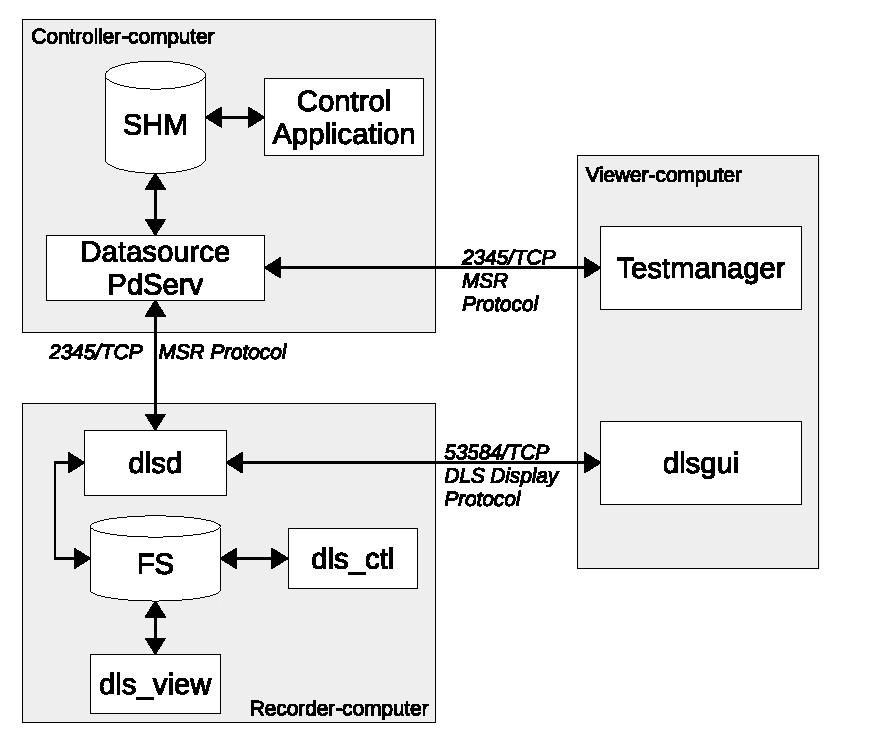
\includegraphics[width=\textwidth]{genpicts/dls-arch.eps}
  \caption{Architecture overview}
  \label{fig:architecture}
\end{figure}


\begin{itemize}

\item There are 3 computers: the controller, the viewer and the recorder.

\item On the controller, the control application exports its
  channels in a shared memory (SHM), then an other process, running
  the PdServer library publishes the channels on the network through the MSR
  protocol (TCP port 2345 by default).
  When the channels are exported on the network any client that
  speaks the MSR protocol can be used to display or record the
  channels.

\item On the recorder, the program \texttt{dlsd} (Data Logging Service
  Daemon) records the selected channels on the filesystem (FS).  The
  program \texttt{dls\_ctl} manages the configuration files for
  \texttt{dlsd} through the filesystem. For example, it can configure
  the list of channels to record.
  \texttt{dls\_view} is a simple viewer that can read directly
  the data files written by \texttt{dlsd}.

\item On the viewer, the program \texttt{testmanager} connects
  directly to the PdServer to display the channels in real-time.  On
  the other hand \texttt{dlsgui} is an advanced data viewer for DLS
  that connects \texttt{dlsd} through a specific network protocol (TCP
  port 5384 by default) to plot recorded data.

\end{itemize}
